\chapter{System description}
\textit{The description below describes the full system to give an overview and provide a project perspective.}

The system comprises a Central data unit and an arbitrary number of sensor nodes. The CDU serves as the main component which have several main functionalities:
\begin{itemize}
	\item Contact all sensor node within fixed time intervals
	\item Store the data locally
	\item Evaluate data and warn patient if necessary
	\item Send data to PC for analysis
\end{itemize}
The CDU supplies a bus where all sensor nodes are interconnected in a serial fashion. This lowers wiring drastically compared to regular sensors.
The CDU continuously request measurement data from each sensor node via the bus. The CDU will be powered by a rechargeable battery with enough power to run the system for atleast a day.\\
The data should be extractable from the CDU to a PC. The connection could be bluetooth, wireless, USB or some other fourth option.

The sensor nodes are application specific IC's and will be covered with epoxy to accommodate the need for hygiene and practically make it possible to wash them. The size of the sensor nodes should be small enough to be of as little discomfort as possible. The sensor nodes should then be built into a sock, shoe or insole.
\begin{figure}[H]
	\centering
	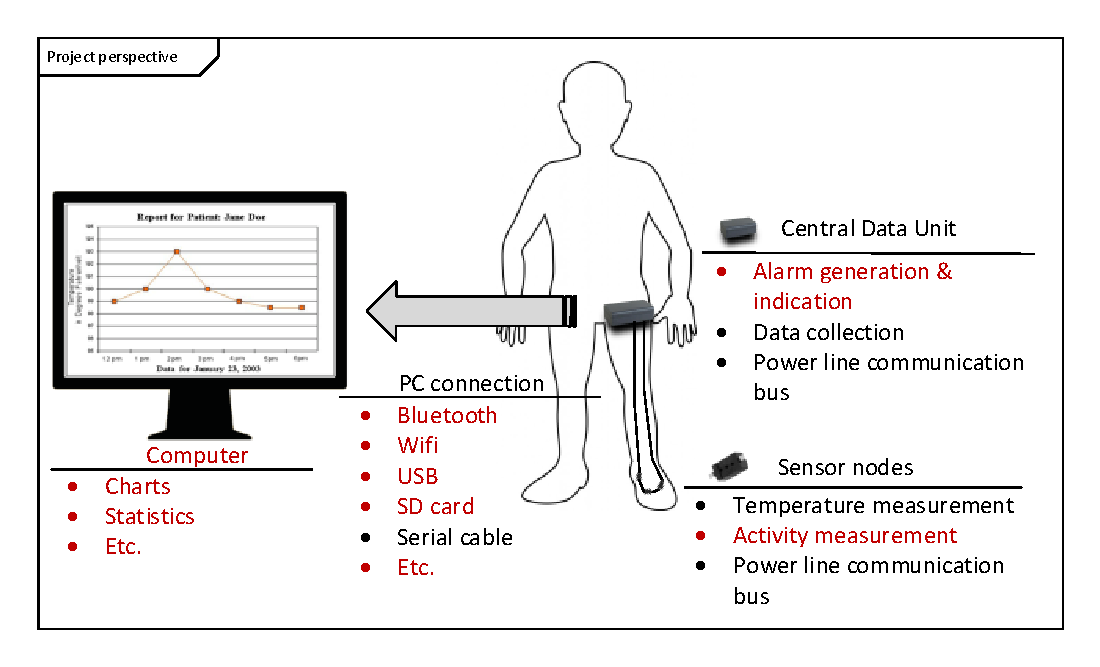
\includegraphics[width=.7\textwidth]{billeder/6Systemdescription/fullsystem_vector}
	\caption{System perspective}
	\label{fig:full_system}
\end{figure}
%%The parts in the figure marked with black is the one were focus is laid upon.